\item The rank of the matrix 
\begin{align*}
\begin{bmatrix} 
1 & -1 & 0 & 0 & 0 \\ 0 & 0 & 1 & -1 & 0 \\ 0 & 1 & -1 & 0 & 0 \\ -1 & 0 & 0 & 0 & 1 \\ 0 & 0 & 0 & 1 & -1 
\end{bmatrix}
\end{align*}
is..........

\item The general solution of the differential equation 
\begin{align}
\frac{d^2 y}{d x^2} + 2 \frac{dy}{dx} - 5y = 0
\end{align}
in terms of arbitrary constants $K_1$ and $K_2$ is 
\begin{enumerate}
\item $K_1e^{(-1 + \sqrt{6})x} + K_2e^{(-1 - \sqrt{6})x}$
\item $K_1e^{(-1 + \sqrt{8})x} + K_2e^{(-1 - \sqrt{8})x}$
\item $K_1e^{(-2 + \sqrt{6})x} + K_2e^{(-2 - \sqrt{6})x}$
\item $K_1e^{(-2 + \sqrt{8})x} + K_2e^{(-2 - \sqrt{8})x}$
\end{enumerate}

\item The smaller angle (in degrees) between the plane 
\begin{align}
x + y + z = 1
\end{align}
\begin{align}
2x - y + 2z = 0
\end{align}
is ...............

\item The residues of a function 
\begin{align*}
f(z) = \frac{1}{(z - 4)(z + 1)^3} 
\end{align*}
are
\begin{enumerate}
\item $\frac{-1}{27}$ and $\frac{-1}{125}$
\item $\frac{1}{125}$ and $\frac{-1}{125}$
\item $\frac{-1}{27}$ and $\frac{1}{5}$
\item $\frac{1}{125}$ and $\frac{-1}{5}$
\end{enumerate}

\item In the circuit shown, V is a sinusoidal voltage source. The current I is in phase with voltage V. The ratio 

$\frac{amplitude of voltage across the capacitor}{amplitude of voltage across the resistor}$

is.................

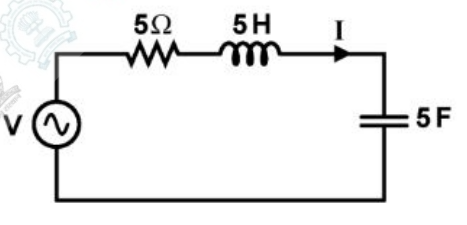
\includegraphics[scale=0.4]{5}

\item A connection is made consisting of resistance A in series with a parallel combination of resistances B and C. Three resistors of value 10 $\Omega$, 5$\Omega$, 2$\Omega$ are provided. Consider all possible permutations of the given resistors into the position A, B, C, and identity the configuration with maximum possible overall resistance, and also the ones with minimum possible overall resistance. The ratio of maximum to minimum values of the resistance (up to second decimal place) is ...........

\item An LTI system with unit sample response 
\begin{align*}
h[n] = 5\delta[n] - 7\delta[n - 1] + 7\delta[n - 3] - 5\delta[n - 4]
\end{align*}
 is a
\begin{enumerate}
\item low-pass filter
\item high-pass filter
\item band-pass filter
\item band-stop filter
\end{enumerate}

\item The input x(t) and the output y(t) of a continuous-time system are related as 
\begin{align}
y(t) = \int_{t - T}^{t}x(u)du
\end{align}
The system is 
\begin{enumerate}
\item linear and time-variant 
\item linear and time-invariant
\item non-linear and time-variant
\item non-linear and time-invariant
\end{enumerate}

\item An n-channel enhancement mode MOSFET is biased at $V_{GS} > V_{TH}$ and $V_{DS} > (V_{GS} - V_{TH})$, where $V_{GS}$ is the gate-to-source voltage, $V_{DS}$ is the drain to source voltage and $V_{TH}$ is the threshold voltage. Considering channel length modulation effect to be significant, the MOSFET behaves as a 
\begin{enumerate}
\item voltage source with zero output impedance
\item voltage source with non-zero output impedance
\item current source with finite output impedance
\item current source with infinite output impedance
\end{enumerate}

\item An $npn$ bipolar junction (BJT) is operating in the active region. If the reverse bias across the base-collector junction is increased,then
\begin{enumerate}
\item the effective base width increases and common-emitter current gain increases
\item the effective base width increases and common-emitter current gain decreases
\item the effective base width decreases and common-emitter current gain increases
\item the effective base width decreases and common-emitter current gain decreases
\end{enumerate}

\item Consider an n-channel MOSFET having width W, length L, electron mobility in the channel $ \mu_n$ and oxide capacitance per unit area $ C_{OX}$. If gate-to-source voltage $V_{GS} = 0.7 V$, drain-to-source voltage $V_{DS} = 0.1 V$, $\mu_{n} C_{OX} = 100\frac{\mu A}{V^2}$, threshold voltage $ V_{TH} = 0.3 V$ and   $\frac{W}{L} = 50$, then the trasconductance $g_{m}$ (in mA/V) is............


\item The output $ V_{o}$ of the diode circuit shown in the figure is connected to an averaging DC voltmeter. The reading on the DC voltmeter in volts, neglecting the voltage drop across the diode, is ..........

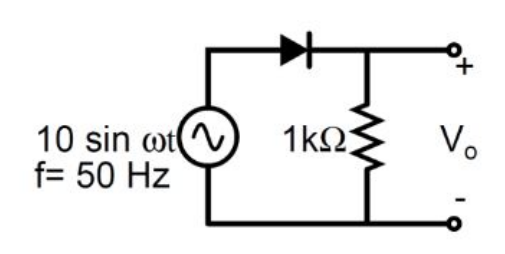
\includegraphics[scale=0.4]{12}

\item In the figure, D1 is a real silicon $pn$ junction diode with a drop of $0.7V$ under forward bias condition and D2 is a Zener diode with breakdown voltage of $-6.8 V$. The input $ V_{in}(t)$ is a periodic square wave of period T, whose one period is shown in the figure.

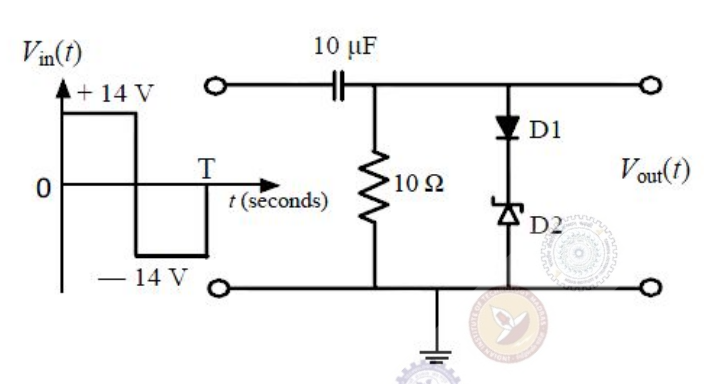
\includegraphics[scale=0.3]{13}

Assuming $10\tau << T$, where $\tau$ is the time constant of the circuit, the maximum and minimum values of the output waveform are respectively.
\begin{enumerate}
\item 7.5V and -20.5V
\item 6.1V and -21.9V
\item 7.5V and -21.2V 
\item 6.1V and -22.6V
\end{enumerate}

\item Consider the circuit shown in the figure. Assume base-to-emitter voltage $ V_{BE}$ = 0.8 V and common-base current gain $(\alpha)$ of the transistor is unity 

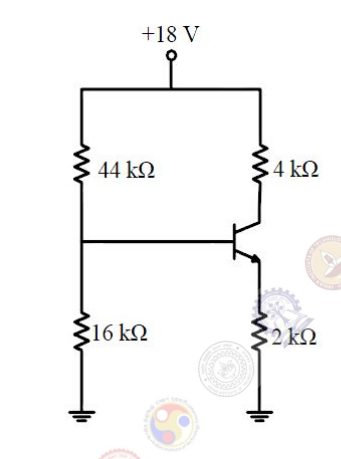
\includegraphics[scale=0.5]{14}

The value of the collector-to-emitter voltage $V_{CE}$ (in volt) is .........

\item For the circuit shown in the figure, P and Q are the inputs and Y is the output.

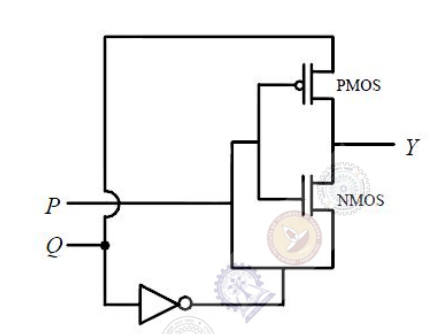
\includegraphics[scale=0.3]{15}

The logic implemented by the circuit is 
\begin{enumerate}
\item XNOR
\item XOR
\item NOR
\item OR
\end{enumerate}

\item Consider the circuit shown in the figure.

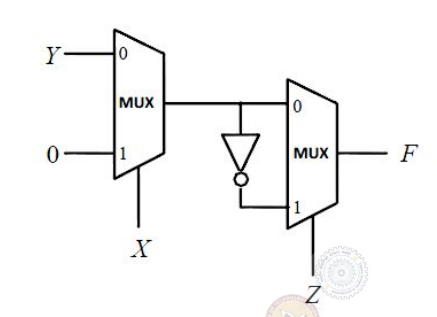
\includegraphics[scale=0.3]{16}

The Boolean expression F implemented by the circuit is 
\begin{enumerate}
\item $\overline{X} \overline{Y} \overline{Z} + XY + \overline{Y}Z$ 
\item $\overline{X} Y \overline{Z} + XZ + \overline{Y}Z$
\item $\overline{X} Y \overline{Z} + XY + \overline{Y}Z$
\item $\overline{X} \overline{Y} \overline{Z} + XZ + \overline{Y}Z$
\end{enumerate}

\item In a DRAM,
\begin{enumerate}
\item periodic refreshing is not required 
\item information is stored in a capacitor
\item information is stored in a latch
\item both read and write operations can be performed simultaneously
\end{enumerate}

\item For the system shown in the figure, $\frac{Y(s)}{X(s)}$ =...........

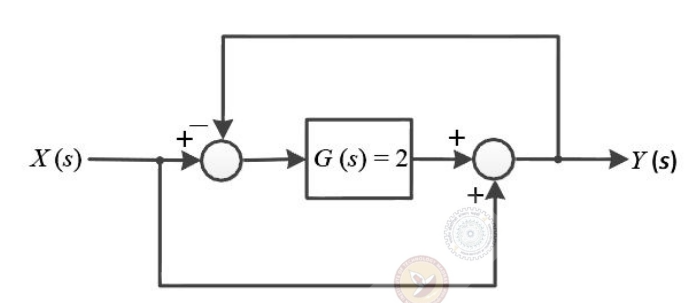
\includegraphics[scale=0.3]{18}

\item Consider the state realization
\begin{align*} 
\begin{bmatrix} 
x_{1}(t) \\ x_{2}(t)
\end{bmatrix} = 
\begin{bmatrix}
0 & 0 \\ 0 & -9
\end{bmatrix}
\begin{bmatrix}
x_{1}(t) \\ x_{2}(t)
\end{bmatrix} +
\begin{bmatrix}
0 \\ 45
\end{bmatrix}
u(t), 
\end{align*}
with the initial condition
\begin{align*} 
\begin{bmatrix}
x_{1}(0) \\ x_{2}(0)
\end{bmatrix} =
\begin{bmatrix}
0 \\ 0,
\end{bmatrix}
\end{align*}
where u(t) denotes the unit step function. The value of
\begin{align*}
\lim_{t \to \infty}|\sqrt{x^{2}_{1}(t) + x^{2}_{2}(t)}| = 
\end{align*}

\item Which of the following statements is incorrect?
\begin{enumerate}
\item Lead compensator is used to reduce the settling time.
\item Lag compensator is used to reduce the steady state error.
\item Lead compensator may increase the order of a system.
\item Lag compensator always stabilizes an unstable system.
\end{enumerate}

\item Which of the following graphs shows the Shannon capacity (channel capacity) in bits of a memoryless binary symmetric channel with crossover probability p?

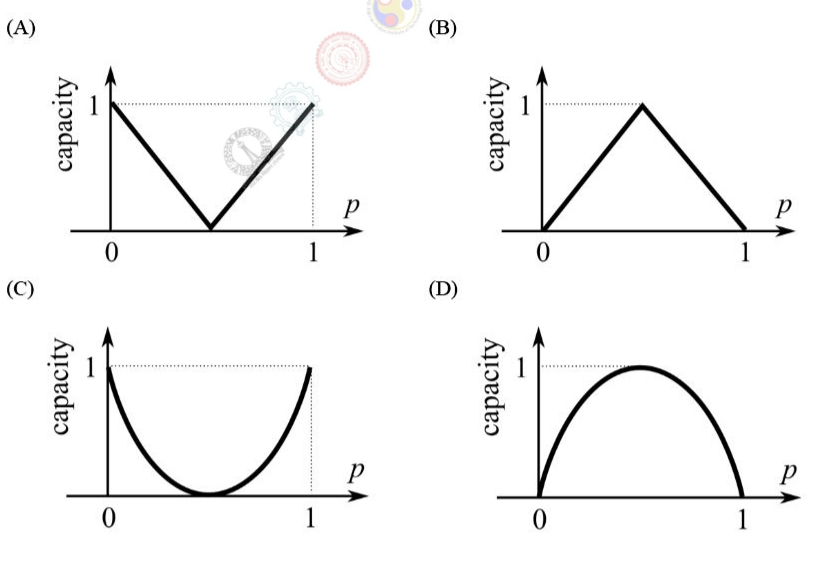
\includegraphics[scale=0.28]{21}

\item Consider the random process
\begin{align*}
X(t) = U + Vt,
\end{align*}
where U is a zero-mean Gaussian random variable and V is a random variable uniformly distributed between 0 and 2. Assume that U and V are statistically independent. The mean value of the random process at t = 2 is .............

\item A sinusoidal message signal is converted to a PCM signal using a uniform quantizer. The required signal-to-quantization noise ratio (SQNR) at the output of the quantizer is 40 dB. The minimum number of bits per sample needed to achieve the desired SQNR is .............


\item Two conducting spheres $S_1$ and $S_2$ of radii a and $(b > a)$ respectively, are placed far apart and connected by a long, thin conducting wire, as shown in the figure.

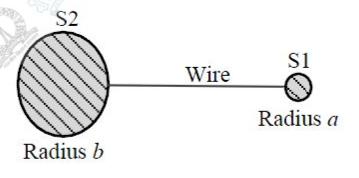
\includegraphics[scale=0.5]{24}

For some charge placed on this structure, the potential and surface electric field on $S_{1}$ are $V_{a}$ and $E_{a}$, and that on $S_{2}$ are $V_{b}$ and $E_{b}$, respectively. Then, which of the following is CORRECT?
\begin{enumerate}
\item $V_{a} = V_{b}$ and $E_{a} < E_{b}$
\item $V_{a} > V_{b}$ and $E_{a} > E_{b}$
\item $V_{a} = V_{b}$ and $E_{a} > E_{b}$
\item $V_{a} > V_{b}$ and $E_{a} = E_{b}$
\end{enumerate}

\item A two-wire transmission line terminates in a television set. The VSWR measured on the line is 5.8. The percentage of power that is reflected from the television set is............


\item The values of the integrals
\begin{align*}
\int_{0}^{1}\left(\int_{0}^{1}\frac{x - y}{(x + y)^{3}}dy\right)dx
\end{align*}
and
\begin{align*}
\int_{0}^{1}\left(\int_{0}^{1}\frac{x - y}{(x + y)^{3}}dx\right)dy
\end{align*}
are
\begin{enumerate}
\item same and equal to 0.5
\item same and equal to -0.5
\item 0.5 and -0.5, respectively
\item -0.5 and 0.5, respectively
\end{enumerate}

\item An integral I over a counter-clockwise circle C is given by
\begin{align*}
\int_{C}^{}\frac{z^2 - 1}{z^2 + 1}e^z dz
\end{align*} 
If C is defined as $|z| = 3$, then the value of I is 
\begin{enumerate}
\item $\pi i \sin(1)$
\item -2$\pi i \sin(1)$
\item -3$\pi i \sin(1)$
\item -4$\pi i \sin(1)$
\end{enumerate}

\item If the vector function 
\begin{align*}
\overrightarrow{F} = \hat{a_x}(3y - k_1z) + \hat{a_y}(k_2x - 2z) - \hat{a_z}(k_3y + z)
\end{align*}
is irrotational, then the values of the constants $k_1$, $k_2$ and $k_3$, respectively, are
\begin{enumerate}
\item 0.3, -2.5, 0.5
\item 0.0, 3.0, 2.0
\item 0.3, 0.33, 0.5
\item 4.0, 3.0, 2.0
\end{enumerate}

\item Passengers try repeatedly to get a seat reservation in any train running two stations until they are successful. If there is $40\%$ chance of getting reservation in any attempt by a passenger, then the average number of attempts that passengers need to make to get a seat reserved is ..........

\item The minimum value of the function 
\begin{align*}
f(x) = \frac{1}{3}x(x^2 -3)
\end{align*}
in the interval $-100 \leq x \leq 100$ occurs at x = ............

\item The switch in the circuit, shown in the figure, was open for a long time and is closed at t = 0.

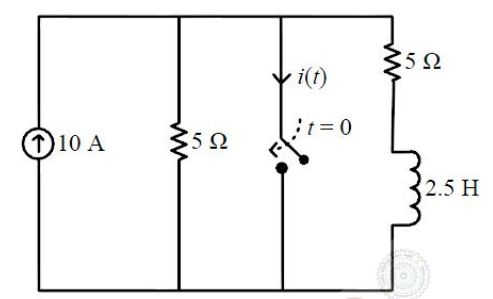
\includegraphics[scale=0.3]{31}

The current $i(t)$ (in ampere) at t = 0.5 seconds is ..............

\item Consider the circuit shown in the figure.

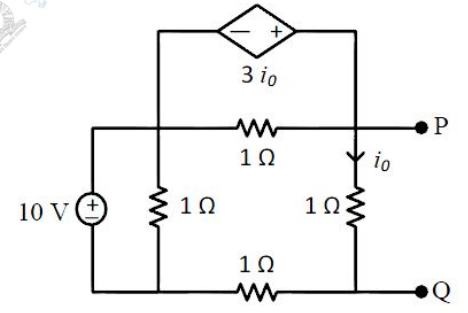
\includegraphics[scale=0.3]{32}

The Thevenin equivalent resistance (in $\Omega$) across P-Q is ................

\item Consider an LTI system with magnitude response
\begin{align*}
|H(f)| = 
\left\lbrace
\begin{array}{ll}
      1 - \frac{|f|}{20}, |f| \leq 20\\
      0, |f| > 20
\end{array}
\right\rbrace
\end{align*}
If the input to the system is 
\begin{align*}
x(t)=8\cos (20 \pi t + \frac{\pi}{4} + 16\sin(40 \pi t + \frac{\pi}{8} \\+ 24\cos(80 \pi t + \frac{\pi}{16}
\end{align*}
then the average power of the output signal $y(t)$ is ..........

\item The transfer function of a causal LTI system is $H(s)=\frac{1}{s}$. If the input to the system is 
\begin{align*}
x(t) = [\frac{\sin(t)}{\pi t}]u(t),
\end{align*}
where $u(t)$ is a unit step function, the system output $y(t)$ as $t \to \infty$ is.............

\item Consider the parallel combination of two LTI systems shown in the figure.

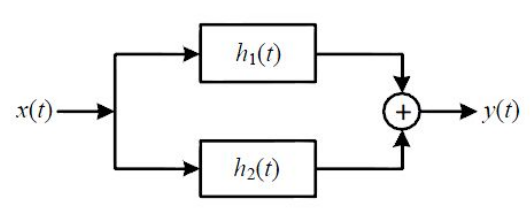
\includegraphics[scale=0.4]{35}

The impulse responses of the systems are 
\begin{align*}
h_{1}(t) = 2\delta(t + 2) - 3\delta(t + 1)
\end{align*}
\begin{align*}
h_{2}(t) = \delta (t - 2).
\end{align*}
If the input $x(t)$ is a unit step signal, then the energy of $y(t)$ is.........


\item A MOS capacitor is fabricated on p-type Si(Silicin) where the metal work funtion is 4.1eV and electron affinity of Si is 4.0eV. $E_{C} - E_{F} = 0.9 eV$, where $E_{C}$ and $ E_{F}$ are the conduction band minimum and the Fermi energy levels of Si, respectively. Oxide $\epsilon_r = 3.9$, $\epsilon_o = 8.85 \times 10^{-14}F/cm$ oxide thickness 
$t_{ox} = 0.1 \mu m$ and electronic charge $q = 1.6 \times 10^{-19} C$. If the measured flat band voltage of this capacitor is -1 V, then the magnitude of the fixed charge at the oxide-semiconductor interface, in $nC/cm^2$,is ..............

\item For a particular intensity of incident light on a silicon $pn$ junction solar cell, the photocurrent density 
$(J_{L})$ is 2.5 $\frac{mA}{cm^2}$ and the open-circuit voltage $ V_{oc}$ is 0.451 V. Consider thermal voltage 
$ (V_{T}$ to be 25 mV. If the intensity of the incident light is increased by 20 times, assuming that the temperature remains unchanged, $V_{oc}$ (in volts) will be.............

\item Two n-channel MOSFETs, $T_{1}$ and $T_{2}$, are identical in all respects except that the width of $T_{2}$ is double that of $T_{1}$. Both the transistors are biased in the saturation region of operation, but the gate overdrive voltage $(V_{GS} - V_{TH})$ of $T_{2}$ is double that of $T_{1}$, where $V_{GS}$ and $V_{TH}$ are the gate-to-source voltage and threshold voltage of the transistors, respectively. If the drain current and transconductance of $T_{1}$ are $I_{D1}$ and $g_{m1}$ respectively, the corresponding values of these two parameters for $T_{2}$ are 
\begin{enumerate}
\item $8I_{D1}$ and $2g_{m1}$
\item $8I_{D1}$ and $4g_{m1}$
\item $4I_{D1}$ and $4g_{m1}$
\item $4I_{D1}$ and $2g_{m1}$
\end{enumerate}

\item An abrupt pn junction (located at x = 0) is uniformly doped on both p and n sides. The width of the depletion region is W and the electric field variation in the x-direction is E(X). Which of the following figures represents the electric field profile near the pn junction?

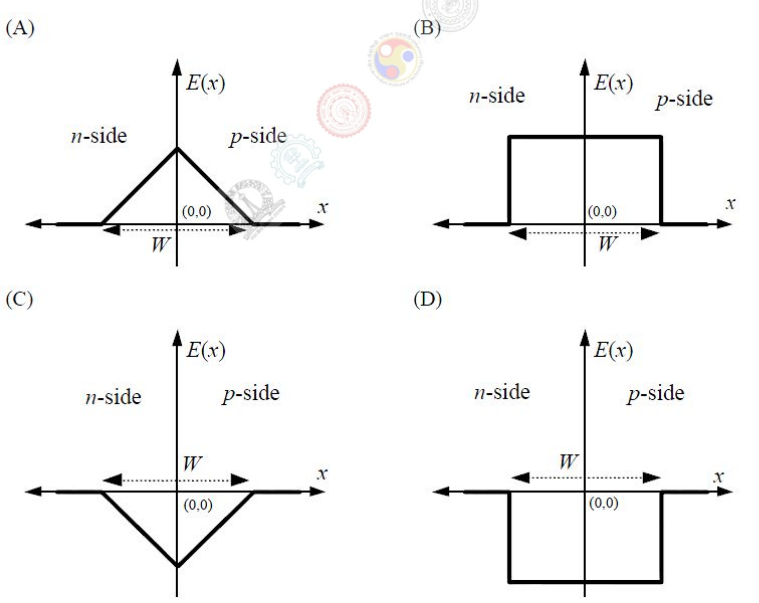
\includegraphics[scale=0.3]{39}

\item Assuming that transistors $M_{1}$ and $M_{2}$ are identified and have a threshold voltage of 1 V, the state of transistors $M_{1}$ and $M_{2}$ are respectively

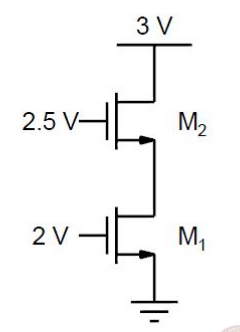
\includegraphics[scale=0.4]{40}

\begin{enumerate}
\item Saturation, Saturation 
\item Linear, Linear
\item Linear, Saturation
\item Saturation, Linear
\end{enumerate}

\item A unity feedback control system is characterized by the open-loop transfer function 
\begin{align*}
G(s) = \frac{2(s + 1)}{s^3 + ks^2 + 2s + 1}
\end{align*}
The value of k for which the system oscillates at 2 rad/s is.............

\item In the circuit shown, transistors $Q_1$ and $Q_2$ are biased at a collector current of 2.6 mA. Assuming that transistor current gains are sufficiently large to assume collector equal to emitter current and thermal voltage of 2.6 mV, the magnitude of voltage gain $\frac{V_o}{V_s}$ in the mid-band frequency range is ........(up to second decimal place).

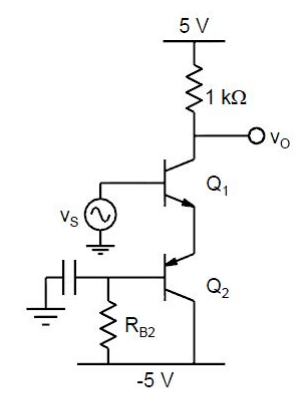
\includegraphics[scale=0.4]{42}

\item In the voltage reference circuit shown in the figure, the op-amp is ideal and the transistors $Q_{1}$, $Q_{2}$,.....,$Q_{32}$ are identical in all respects and have infinitely large values of common-emitter current gain $\beta)$. The collector current $(I_{c})$ of the transistors is related to their base-emitter voltage $(V_{BE})$ by the relation $I_{c} = I_{S} exp(V_{BE}/V_{T})$, where $(I_{s})$ is the saturation current. Assume that the voltage $(V_{p})$ shown in the figure is 0.7 V and the thermal voltage $(V_{p})$ = 26 mV.

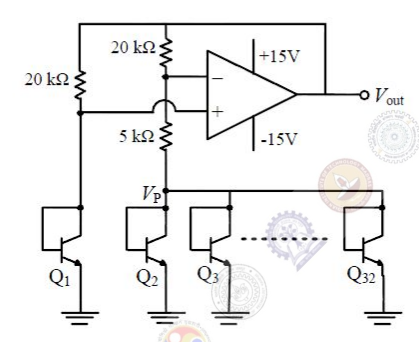
\includegraphics[scale=0.4]{43}

The output voltage $V_{out}$(in volts) is ...........

\item The state diagram of a finite state machine (FSM) designed to detect an overlapping sequence of three bits is shown in the figure. The FSM has an input $'In'$ and an output $'Out'$. The initial state of the FSM is $S_{o}$.

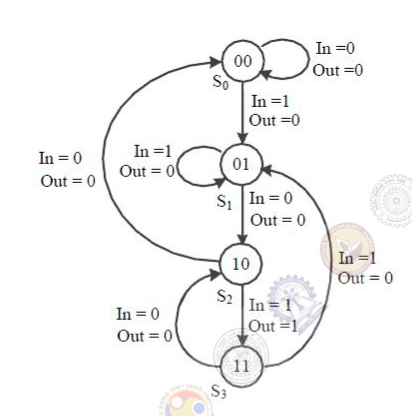
\includegraphics[scale=0.4]{44}

If the input sequence is 10101101001101, starting with the left-most bit, then the number of times $'Out'$ will be 1 is ..........

\item Figure I shows a 4-bit ripple carry adder realized using full address and Figure II shows the circuit of a full-adder (FA). The propagation delay of the XOR, AND and OR gate in Figure II are 20ns, 15ns, and 10ns, respectively. Assume all the inputs to the 4-bit adder are initially reset to 0.

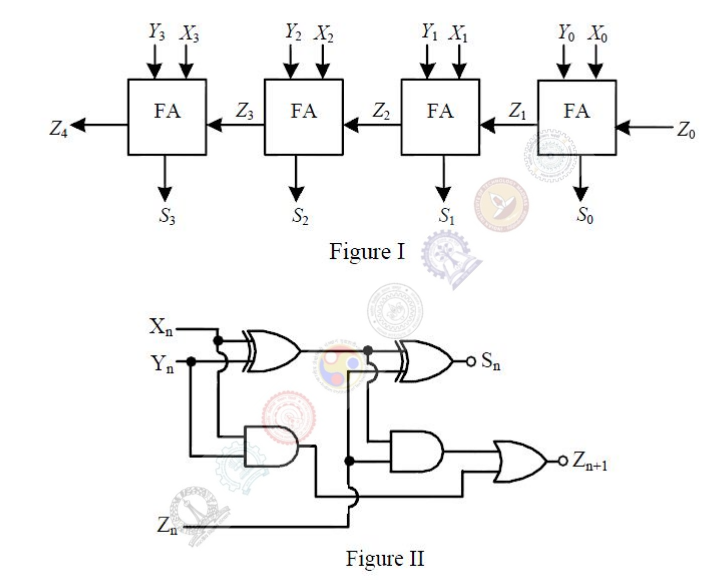
\includegraphics[scale=0.3]{45}

At t=0, the inputs to the 4-bit adder are changed to $X_3X_2X_1X_0 = 1100$, $Y_3Y_2Y_1Y_0 = 0100$ and $Z_O = 1$. The output of the ripple carry will be stable at t (in ns) =.............

\item A programmable logic array (PLA) is shown in the figure.

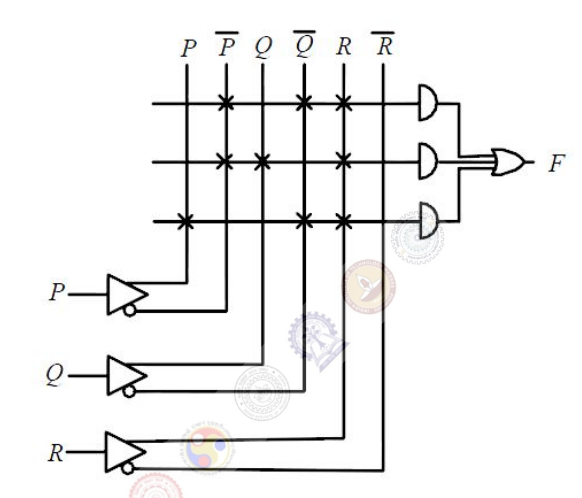
\includegraphics[scale=0.42]{46}

The Boolean function F implemented is 
\begin{enumerate}
\item $\overline{P}$ $\overline{Q}$ R + $\overline{P}$ Q R + P $\overline{Q}$ $\overline{R}$
\item ($\overline{P}$ + $\overline{Q}$ + R ) ($\overline{P}$ + Q + R ) ( P + $\overline{Q}$ + $\overline{R}$)
\item $\overline{P}$ $\overline{Q}$ R + $\overline{P}$ Q R + P $\overline{Q}$ R
\item ($\overline{P}$ + $\overline{Q}$ + R ) ($\overline{P}$ + Q + R ) ( P + $\overline{Q}$ + R)
\end{enumerate}

\item A second-ordered LTI system is described by the following state equations.
\begin{align}
\frac{d}{dt} x_1 (t) - x_2 (t) = 0
\end{align}
\begin{align}
\frac{d}{dt} x_2 (t) + 2 x_1 (t) + 3 x_2 (t) = r(t)
\end{align}
where $x_{1}$ t and $x_{2}$ t are two state variables and r(t) denotes the input. The output c(t)=$x_{1}$ (t). The system is
\begin{enumerate}
\item undamped (oscillatory)
\item underdamped
\item critically damped
\item overdamped
\end{enumerate}

\item A unity feedback control system is characterized by the open-loop transfer function
\begin{align*}
G(s) = \frac{10k(s + 2)}{s^3 + 3s^2 +10}
\end{align*}
The Nyquist path and the corresponding Nyquist plot of G(s) are shown in the figures below.

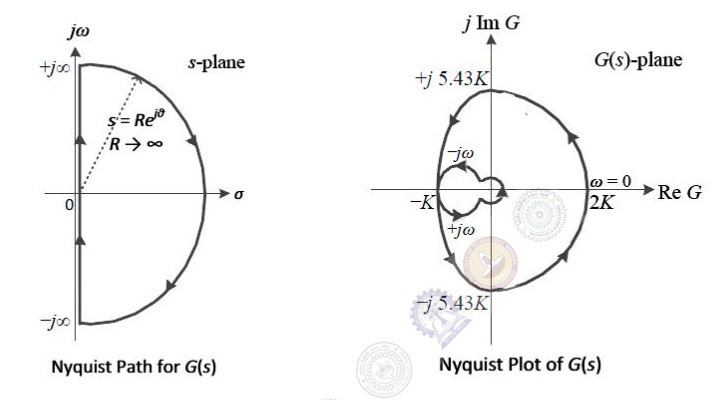
\includegraphics[scale=0.3]{48}

If $0 < k < 1$, then the number of poles of the closed-loop transfer function that lie in the right half of the s-plane is 
\begin{enumerate}
\item 0
\item 1
\item 2 
\item 3
\end{enumerate}

\item The signal $x(t) = \sin(14000\pi t)$, where t is in seconds, is sampled at a rate of 9000 samples per second. The sampled signal is the input to an ideal lowpass filter with frequency response $H(f)$ as follows:
\begin{align*}
H(f) = 
\left\lbrace
\begin{array}{ll}
      1, |f| \leq 12kHz\\
      0, |f| > 12kHz
\end{array}
\right\rbrace
\end{align*}
What is the number of sinusoids in the output and their frequencies in kHz?
\begin{enumerate}
\item Number = 1, frequency = 7 
\item Number = 3, frequencies = 2, 7, 11
\item Number = 2, frequencies = 2, 7
\item Number = 2, frequencies = 7, 11
\end{enumerate}

\item The unmodulated carrier power in an AM tranmitter is 5 kW. This carrier is modulated by a sinusoidal modulating signal. The maximum percentage of modulation is $50\%$. If it is reduced to $40\%$, then the maximum unmodulated carrier power(in kW) that can be used without overloading the transmitter is ..............

\item A modulating signal given by 
\begin{align*}
x(t) = 5 \sin(4 \pi 10^3 t - 10 \pi \cos2 \pi 10^3 t)V
\end{align*}
is fed to a phase modulator with phase deviation constant $k_{p} = 5 rad/V$. If the carrier frequency is 20 kHz, the instantaneous frequency (in kHz) at t = 0.5ms is ..........

\item Consider a binary memoryless channel characterized by the transition probability diagram shown in the figure.

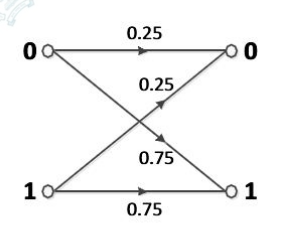
\includegraphics[scale=0.5]{52}

The channel is
\begin{enumerate}
\item lossless
\item noiseless
\item useless
\item deterministic
\end{enumerate}

\item An electron $q_{1}$ is moving in free space with velocity $10^5$ m/s towards a stationary electron $q_{2}$ far away. The closest distance that this moving electron gets to the stationary electron before the repulsive force diverts it path is ...............$ \times 10^{-8}$m.
[Given, mass of electron $m = 9.11 \times 10^{-31}$kg, charge of electron $e = -1.6 \times 10^{-19}$C, and permittivity
$\epsilon_{o} = 1/36 \pi \times 10^{-9}F/m$ 

\item Standard air-filled rectangular waveguides of dimensions a = 2.29 cm and b = 1.02 cm are designed for radar applications. It is desired that these waveguides operate only in the dominant $TE_{10}$ mode with the operating frequency at least $25 \%$ above the cutoff frequency of the  $TE_{10}$ mode but not higher than $95 \%$ of the next higher cutoff frequency. The range of the allowable operating frequency f is ........
\begin{enumerate}
\item $8.19 GHz \leq f \leq 13.1 GHz$
\item $8.19 GHz \leq f \leq 12.45 GHz$
\item $6.55 GHz \leq f \leq 13.1 GHz$
\item $1.64 GHz \leq f \leq 10.24 GHz$
\end{enumerate}

\item The permittivity of water at optical frequencies is 1.75 $\epsilon_0$. It is found that an isotropic light source at a distance d under water forms an illuminated circular area of radius 5 m, as shown in the figure. The critical angle is 
$\theta_c$.

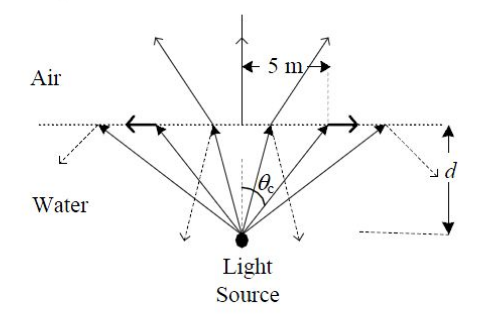
\includegraphics[scale=0.4]{55}

The value of d (in meter) is ...........

\item The ninth and the tenth of this month are Monday and Tuesday............
\begin{enumerate}
\item figuratively
\item retrospectively
\item respectively
\item rightfully
\end{enumerate}

\item It is.............to read this year's textbook ............ the last year's.
\begin{enumerate}
\item easier, than
\item most easy, than
\item easier, from
\item easier, from
\end{enumerate}

\item A rule states that in order to drink beer, one must be over 18 years old. In a bar, there are 4 people, P is 16 years old, Q is 25 years old, R is drinking milkshake and S is drinking a beer. What must be checked to ensure that the rule is being followed ?
\begin{enumerate}
\item Only P's drink
\item Only P's drink and S's age
\item Only S's drink
\item Only P's drink, Q's drink and S's age
\end{enumerate}

\item Fatima starts from point P, goes North for 3 km, and the East for 4 km to reach point Q. She then turns to face point P and goes 15 km in that direction. She then goes North for 6 km. How far is she from point P, and in which direction should she go to reach point P?
\begin{enumerate}
\item 8 km, East
\item 12 km, North
\item 6 km, East
\item 10 km, North
\end{enumerate}

\item 500 students are taking one or more courses out of Chemistry, Physics, and Mathematics. Registration records indicate course enrolment as follows: Chemistry (329), Physics (186), Mathematics (295), Chemistry and Physics (83), Chemistry and Mathematics (217), and Physics and Mathematics (63). How many students are taking all 3 subjects ?
\begin{enumerate}
\item 37
\item 43
\item 47
\item 53
\end{enumerate}

\item "If you are looking for a history of India, or for an account of the rise and fall of the British Raj, or for the reason of the cleaving of the subcontinent into two mutually antagonistic parts and the effects this mutilation will have in the respective sections, and ultimately on Asia, you will not find it in these pages; for though I have spent a lifetime in the country. I lived too near the seat of events , and was too intimately associated with the actors, to get the perspective needed for the impartial recording of these matters."

Which of the following statements best reflects the author's opinion?
\begin{enumerate}
\item An intimate association does not allow for the necessary perspective.
\item Matters are recorded with an impartial perspective.
\item An intimate association offers an impartial perspective.
\item Actors are typically associated with the impartial recording of matters.
\end{enumerate}

\item Each of P, Q, R, S, W, X, Y and Z has been married at most once. X and Y are married and have two children P and Q, z is the grandfather of the daughter S of P. Further, Z and W are married and are parents of R. Which one of the following must necessarily be FALSE?
\begin{enumerate}
\item X is the mother-in law of R
\item P and R are not married to each other
\item P is a son of X and Y
\item Q cannot be married to R
\end{enumerate}

\item 1200 men and 500 women can build a bridge in 2 weeks. 900 men and 250 women will take 3 weeks to build the same bridge. How many men will be needed to build the bridge in one week?
\begin{enumerate}
\item 300
\item 3300
\item 3600
\item 3900
\end{enumerate}

\item The number of 3-digit numbers such that the digit 1 is never to the immediate right of 2 is 
\begin{enumerate}
\item 781
\item 791
\item 881
\item 891
\end{enumerate}

\item A contour line joins locations having the same height above the mean sea level. The following is a contour plot of a geographical region. Contour lines are shown at 25 m intervals in this plot.

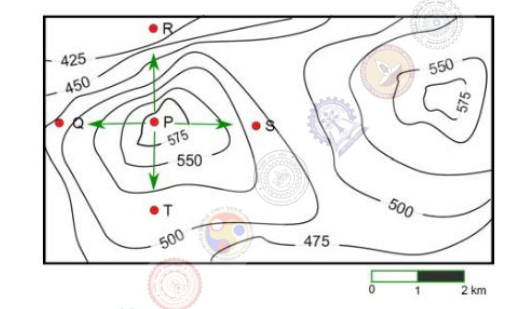
\includegraphics[scale=0.4]{65}

\begin{enumerate}
\item P to Q
\item P to R
\item P to S
\item P to T
\end{enumerate}